\section{Problemområde}

Systemet har forskellige emner der skal modelleres, derfor skal problemområdet analyseres.
Problemområdet defineres ifølge \textit{Objekt Orienteret Analyse \& Design}\citep{OOA&D2001} som:

\textit{``Den del af omgivelserne, der administreres, overvåges eller styres ved hjælp af et system.''}

Systemet skal holde styr på tilbud, generelle varer, og opskrifter.
Der skal registreres hvis en varer er på tilbud, hvor denne vare er på tilbud, og om brugeren ønsker at købe varen.
Opskrifterne har en liste over ingredienser, som består af varer.
Opskrifterne skal også kunne blive vurderet, så systemet kan anbefale lignende opskrifter til brugeren.
Varer skal også kunne overvåges, og systemet skal give besked til brugeren når et tilbud på varen dukker op.
Systemet skal kunne medbringes på indkøbsturen, og her skal tilbudene og varerne fra systemet kunne indgå på en indkøbsliste.

Med disse informationer kan systemet hjælpe brugeren til at finde billige varer i bestemte butikker, og eventuelt anbefale opskrifter der bruger disse tilbudsvarer.
I de følgende afsnit vil disse emner blive beskrevet vha. klassebeskrivelser, en hændelsestabel, og et klassediagram.

\subsection{Struktur}\label{sec:struktur}
For at skabe et overblik over hvilke objekter der findes i problemområdet, samt hvilke klasser disse tilhører og at til sidst kunne kæde dette sammen med hændelser i problemområdet, foretages først en analyse af strukturen.\\

\begin{figure}
	\centering
		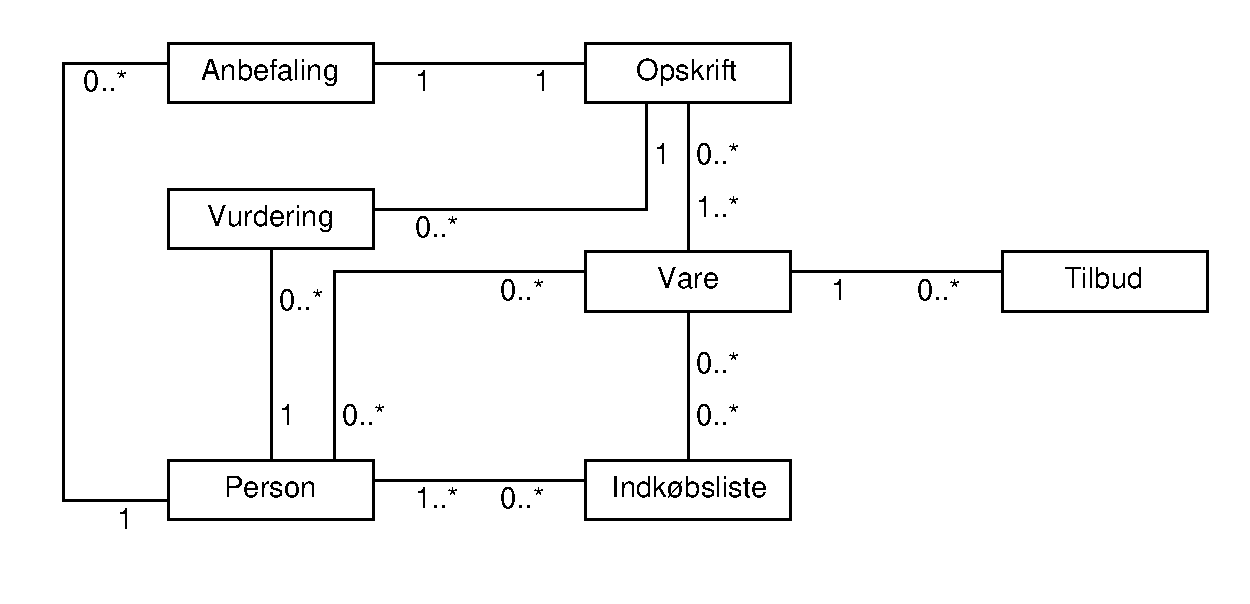
\includegraphics[scale=0.6]{images/Diagrams/klassediagram_model_simple.pdf}
	\caption{Klassediagram over problemområdet.}
	\label{figur:PDklasse}
\end{figure}

Dette er beskrevet vha. et klassediagram som ses på Figur \ref{figur:PDklasse}, dette beskriver forholdet mellem de forskellige objekter som findes i problemområdet til indkøb og madlavning. Den følgende tekst uddyber figuren.

Personer i indkøbssituationer kan lave indkøbslister, disse indkøbslister kan været ejet og administreret af en enten en eller flere personer.
En indkøbsliste kan bestå an ingen til en højt antal varer.
En vare kan komme fra tre forskellige steder.
Varer kan stamme fra et tilbud, eller de kan være ingredienser fra en opskrift.
Hvis en vare ikke er nogle af disse ting, er varen blot generisk, det vil sige en vare uden forhold til et tilbud eller en opskrift.
Et tilbud består som tidligere nævnt af en vare.
Et tilbud har nogle attributter der beskriver varen, samt pris og lignende.
En avis består af minimum et tilbud men har oftest en samling af tilbud, og en sådan avis har et tilhørsforhold der består af en butik, som udgiver avisen med tilbudene i.\\
Som tidligere nævnt kan en vare også udgøre en ingrediens i en opskrift.
En opskrift består af en eller flere ingredienser, beskrevet som varer.
En person i problemområdet kan, vurderer den en opskrift, for at beskrive hvor tilfredsstillende de fandt opskriften.
En person vil maksimalt kunne give hver opskrift en vurdering, men kan også undlade at vurdere en opskrift.

\subsection{Klasser}
De forskellige klasser som beskrevet i \myref{sec:struktur} vil beskrives ydeligere i dette afsnit.

\textbf{Opskrift:}
Denne klasse indeholder en titel på opskriften, en liste over ingredienser, forberedelsestid samt en fremgangsmåde. Klassen modellerer hændelserne der sker når en bruger vurdere og vælger en opskrift.

\textbf{Vare:}
Denne klasse indeholder et navn, en kategori f.eks. kød, mejeri, grønt m.m. samt information om varen er på tilbud. Denne klasse bruges hver gang en bruger tilgår en opskrift, eller bruger indkøbslisten.

\textbf{Klient:}
Denne klasse indeholder et navn/ID såvel som en indkøbsliste, en overvågnings, grupper som klienten er medlem af, samt klientens personlige præferencer. Herudover findes der også en liste over varer, klienten kan være specielt interesseret i, og derfor overvåger for tilbud. Klassen bruges når der afgives vurderinger og valg af opskrifter, eller når indkøbslister oprettes.

\textbf{Tilbud:}
Denne klasse indeholder alt relevant information om de enkelte tilbud, dette indebærer tilbudsperiode, tilbudspris, butikskæden hvor varen er på tilbud, hvilken vare er på tilbud, mærket på varen samt varens enhed. Klassen benyttes når en butikskæde udgiver nye tilbud, og når tilbudene føjes til indkøbslisten.

\textbf{Tilbudsavis:}
Denne klasse indeholder alle tilbud for en given kæde og består således af et kædens navn, en liste over deres aktive tilbud samt tilbudsperioden på disse tilbud. Tilbudsaviser udkommer forskellige dage på ugen, og benyttes ved hændelsen når en ny avis udkommer.

\textbf{Indkøbsliste:}
Denne klasse indeholder en liste over vare og tilbud som klienten har sat på sin liste. Desuden indeholder den også information om hvilke klienter der kan se listen, når den er delt med andre. Indkøbslisten bruges i det den bliver oprettet, slettet eller når varer tilføjes.


\subsection{Hændelser}
Vi har fundet frem til de forskellige hændelser der sker i problemområdet.
Ud fra disse laves en hændelsestabel, der beskriver hvilke klasser forskellige hændelser påvirker.
Formålet med at identificere hændelserne samt at analysere disse i en hændelsestalbel, er at forstå problemområdet bedre og dermed hjælpe med forståelsen for hvordan en løsning ville kunne udarbejdes for at afhjælpe de problemer der findes i problemområdet. Desuden kan tabellen hjælpe med strukturen på klasserne.
Hvis 2 klasser har alle de samme hændelser, kan der ofte foretages ændringer og dermed opnå en bedre struktur.

\begin{table}[H]
  \centering
    \colorlet{shadecolor}{gray!40}
    \rowcolors{1}{white}{shadecolor}
      \begin{tabular}{l|lccccccc}
      %\hline
       								& \rot{Tilbud}  & \rot{Indkøbsliste} & \rot{Opskrift} & \rot{Vare} & \rot{Person}& \rot{Vurderinger} \\ \hline
      Vare tilføjet til indkøbsliste&               & +      &          & +     & +     &   \\ 
      Vare fjernet fra indkøbsliste	&              	& +      &          & +     & +     &   \\ 
      Vare aftjekket på indkøbsliste&               & +      &          & +     & +     &   \\ 
      Opskrift valgt ???       		& +             & +      &          & +     & +     &   \\ 
      Tilbud oprettet        		& +            	& +      & +        & +     &       &   \\ 
      Tilbud aktiveret        		& +            	& +      & +        & +     &       &   \\ 
      Tilbud udgået          		& +        		& +      & +     	&       &       &   \\ 
      Vare tilføjet til overvågning & +          	&        &          & +     & +     &   \\ 
      Vare fjernet fra overvågning  & +          	&        &          & +     & +     &   \\ 
      Overvågningsvare på tilbud    & +  			&		 &			& + 	& +		&	\\
      Del indkøbsliste       		&               & +      &          &       & +     &   \\ 
      Indkøbsliste oprettet  		&              	& +      &          &       & +     &   \\ 
      Indkøbsliste slettet  		&             	& +      &          &       & +     &   \\ 
      Vurdering givet				&             	&        & +        &       & +		& + \\
      Anbefaling givet				&				&		 & +		&		& +		& + \\
      
    \end{tabular}
  \caption{Hændelsestabel. Viser hvilket klasser, problemområdets hændelser påvirker.}\label{tabel:haendelsestabel}
\end{table}


Hændelsestabellen i Tabel \ref{tabel:haendelsestabel} viser både hvilke hændelser der findes i problemområdet, samt hvilke klasser de påvirker.
Hvis tabellen læses vandret kan det ses at klasser der bliver påvirket af mange hændelser er klasser som "Indkøbsliste", "Vare" og "Bruger".


Ud fra denne analyse dannes et overblik, over klassernes interne interaktion, såvel som hvilke hændelser, involverer hvilke klasser.
Denne information kan vi bruge som udgangspunkt til at lave klassediagram, og tilstandsdiagram i anvendelsesområdet.
I sidste ende giver dette en beskrivelse af systemets overordnede struktur.
